\documentclass{bioinfo}
\copyrightyear{2016} \pubyear{2016}

\access{Advance Access Publication Date: Day Month Year}
\appnotes{Manuscript Category}

\begin{document}
\firstpage{1}

\subtitle{Data and text mining}

\title[mimic-code]{MIMIC Code Repository: Tools For Deriving Clinical Concepts}
\author[Johnson \textit{et~al}.]{Alistair E. W. Johnson\,$^{\text{\sfb 1,}*}$ and Tom J. Pollard\,$^{\text{\sfb 1}}$}
\address{$^{\text{\sf 1}}$Institute of Medical Engineering \& Science, Massachusetts Institute of Technology, Cambridge, 02139, USA %and \\
%$^{\text{\sf 2}}$Department, Institution, City, Post Code, Country.
}

\corresp{$^\ast$To whom correspondence should be addressed.}

\history{Received on XXXXX; revised on XXXXX; accepted on XXXXX}

\editor{Associate Editor: XXXXXXX}

\abstract{\textbf{Motivation:} Secondary analysis of electronic health records is an important method for gaining insight into clinical care. Retrospective studies frequently require similar clinical concepts, so there is benefit in providing open, standardized tools for deriving these concepts to ensure the consistency and efficiency of future studies.\\
\textbf{Results:} We present the MIMIC Code Repository, a collection of open source code for deriving clinical concepts using the MIMIC Critical Care Database. Concepts include severity of illness scores, organ failure indices, and duration of treatments such as ventilation and dialysis. \\
\textbf{Availability:} The MIMIC Code Repository is in active development on GitHub. All code is made available under a permissive MIT license unless otherwise indicated.\\
\textbf{Contact:} \href{aewj@mit.edu}{aewj@mit.edu}\\
\textbf{Supplementary information:} Supplementary data are available at \textit{Bioinformatics} online.}

\maketitle

\section{Introduction}

\subsection{Intensive care data}

There is substantial heterogeneity in intensive care populations - for example in aspects of patient physiology, presence of disease, and intervention types - which presents a significant challenge in terms of understanding the relationships between provision of care and patient outcomes. As a result, the benefit of many widely-practiced treatments and interventions remains unproven [REFS: VINCENT etc].

Vast quantities of data are routinely collected by modern hospital monitoring systems, particularly in intensive care units where patients frequently suffer organ failure and require close observation. There is optimism that increasing availability of large scale clinical databases will offer opportunities to overcome many of the challenges associated with heterogeneity and offer new insights into critical care medicine [REF: BIG DATA etc]. 

One such database is the Medical Information Mart for Intensive Care (MIMIC-III), a large database collected from patients admitted to intensive care units in the Beth Israel Deaconess Medical Center, Boston, MA, USA \cite{mimiciii}. The latest version of MIMIC-III, v1.3, houses data spanning 11 years between 2001 and 2012, and is made freely available to researchers upon signing of a data use agreement and proof of a human studies training course. 

MIMIC-III is an unmatched research resource in the area of critical care informatics that not only promotes crowdsourcing of knowledge generation but, more importantly, allows investigators to easily reproduce and expand upon results that utilize the data. [Briefly say here that in the past people have not shared their code systematically, which is bad. Leads on to next section.]

% Analysis of the data collected by these systems has the potential to increase medical knowledge, taking us towards improved care and patient outcomes.

% help to provide a solution to... Analysis often requires matching patients based on severity, selecting cohorts based on presence of comorbidities, etc. There is therefore benefit in developing reusable code for... Quantifying the severity of illness for a patient is an integral part of retrospective analysis as it allows for investigation of concepts of interest in comparable patient populations. 

% Set out some of the problems and our knowledge gaps. Emphasise importance of research. For example, preventable mortality, reducing length of stay, preserving resources etc. Introduce some studies that have used MIMIC. Explain that code has been written independently on each occasion. 

% To address these gaps in our knowledge, key steps are needed. Available data. Studies that can be reviewed and improved and repeated over new datasets. Facilitated by code sharing etc..

\subsection{MIMIC Code Repository}

Analysis of critical care data often requires definition of clinical concepts, such as severity of illness scores, organ failure indices, and duration of treatments including ventilation and dialysis. Typically the code used to generate these concepts is generated by the researcher and often not widely shared for reuse or validation. The result is that work is not easily reviewed and reused, leading to inconsistent approaches between projects, repeated work, and increased probability of errors in the extraction process. 

The MIMIC Code Repository helps to address these issues by providing a centralised and collaborative codebase for the research community. By allowing researchers to collaboratively develop, share, and review code, the repository helps to standardize the definition of key clinical concepts, promotes continuous review and improvement, and facilitates future studies on the MIMIC-III database. 

\begin{methods}
\section{Methods}

\subsection{Deriving clinical concepts}

The MIMIC Code Repository is seeded with code for generating clinical concepts that are widely used in research studies. A large proportion of the code is written in structured query language (SQL), primarily tailored to the PostgreSQL database system. For example, code has been provided for deriving:

\begin{itemize}
\item the Angus criteria for sepsis [REF TO ANGUS]. Sepsis is a serious illness caused by infection and is a major focus of clinical research [REF TO PAPERS USING ANGUS].
\item severity of illness scores, such as the Simplified Acute Physiology Score II (SAPS-II), the Oxford Acute Severity of Illness Score (OASIS), and the Acute Physiology Score III (APS III) [REFS]. These scores are often used to adjust for severity of illness in clinical studies to support analysis across comparable patient populations [REFS] .
\item additional clinical concepts such as the Sequential Organ Failure Assessment (SOFA) and the Elixhauser Comorbidity Index [REFS].
\item detail relating to patient treatment, such as length of vasopressor use and start and stop times for mechanical ventilation [REFS].
\end{itemize}

Add more detail here. Perhaps switch bullet point list above into separate paragraphs. The performance of two different implementations of the SOFA score in discriminating hospital mortality is shown in Figure \ref{fig:SevScoresOverTime}.

A prerequisite for using much of the code in the MIMIC Code Repository is access to the MIMIC-III Database, so we provide scripts to enable researchers to build local copies of the MIMIC database in a variety of database systems, including PostgreSQL, MySQL, Oracle, and MonetDB. The scripts create table structure, load data, and provide views for ease of interpretation. 

Additionally, we seek to provide introduction to the data. Tutorials are provided to give new users and introduction to the MIMIC database. A 'cookbook' of sample code is provided to introduce new users to the database in a friendly way. Ipython notebooks.

% Explain importance of the code. Why is it necessary. Who will use it? More detail about specific issue being addressed by the code. more detail about performance of the code.

% Studying the impact of treatment on patient health or adjusting for the use of treatment during a patient's care is a common task in secondary analysis of electronic health records. The MIMIC Code Repository provides start and stop times for mechanical ventilation, dialysis, and various vasopressors. An example of these durations is provided in Figure \ref{fig:treatment}.

% There are five severity of illness scores currently implemented in the MIMIC Code Repository: APS-III \cite{aps}, SAPS \cite{saps}, SAPS-II \cite{sapsii}, SOFA \cite{sofa} and OASIS \ref{oasis}. The performance of these scores in discriminating hospital mortality is shown in Figure \ref{fig:SevScoresOverTime}. More detailed comparison of the severity scores is provided in the supplementary material.

\begin{figure}[!tpb]%figure1
\centerline{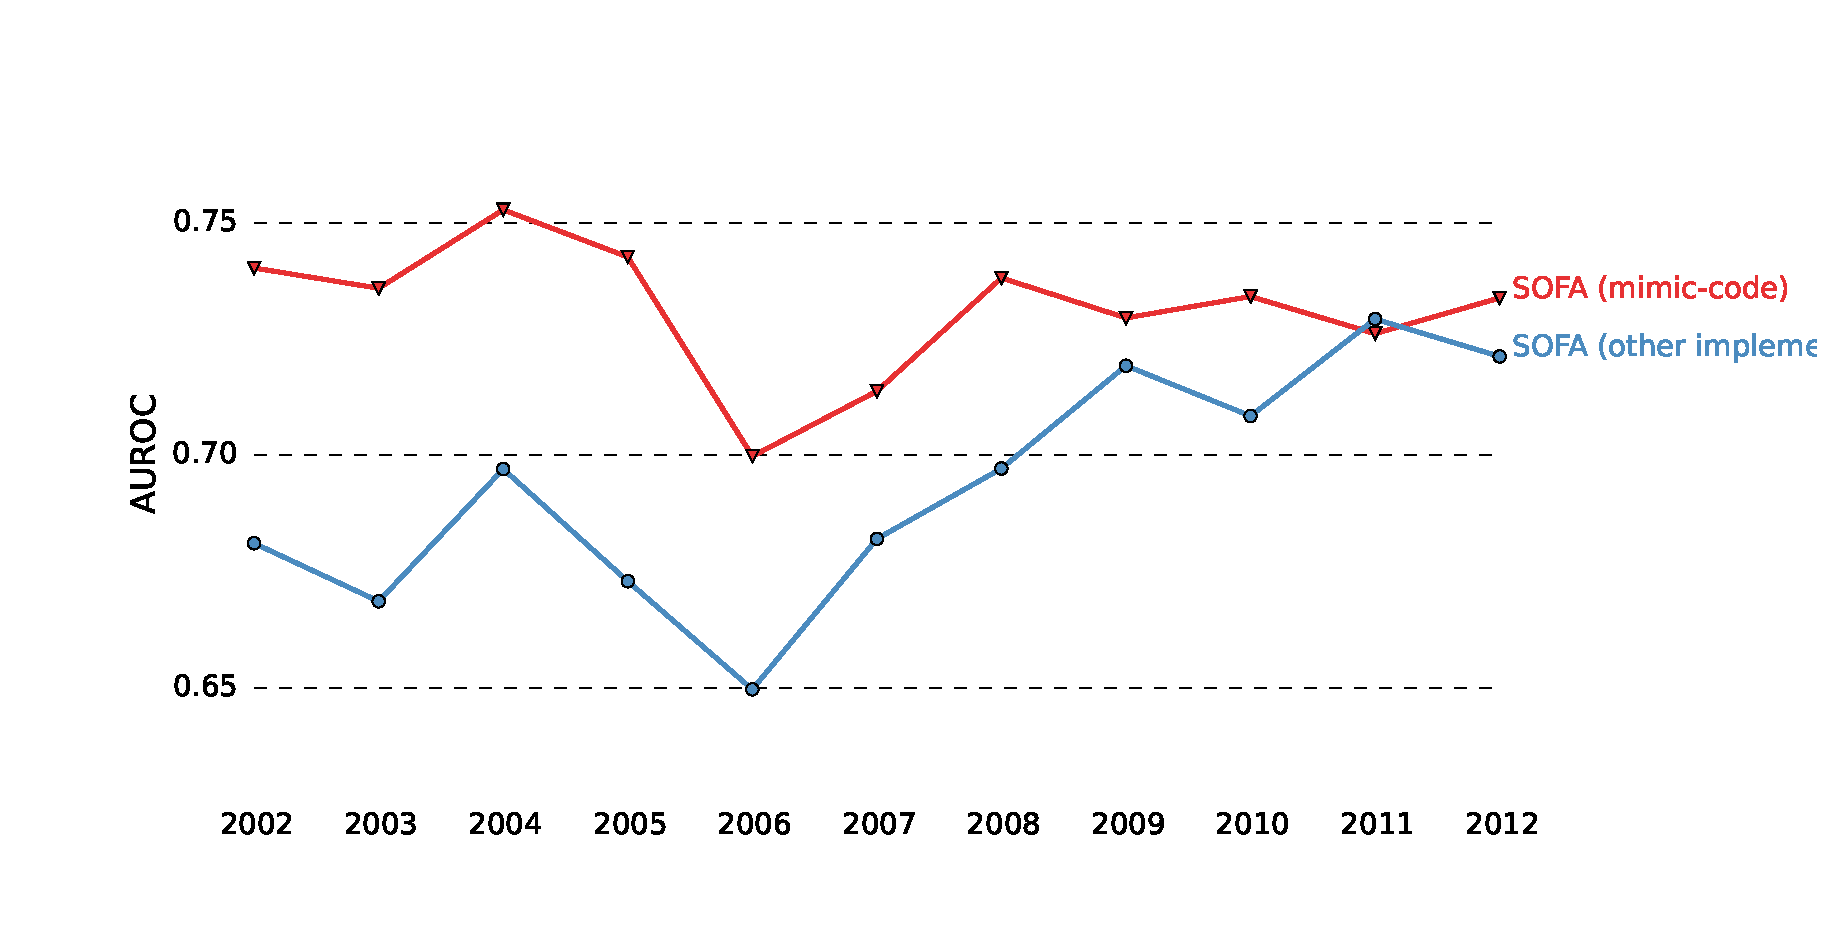
\includegraphics[width=0.5\textwidth]{SOFA.eps}}
\caption{Discrimination of two implementations of SOFA across fiscal years as measured by the area under the receiver operator characteristic curve (AUROC).}\label{fig:SevScoresOverTime}
\end{figure}

% In addition, scores used to measure the failure of a specific organ are also available for the hepatic (MELD \cite{meld}) and renal (KDIGO \cite{kdigo}, RIFLE \cite{rifle}) systems.

\subsection{Collaboration}

Conducting effective clinical research calls for a broad range of knowledge, covering areas such as clinical practice, data collection processes, and analytical methods. For this reason, we believe that it is important to nurture collaboration between disciplines including caregivers, computer scientists, and data analysts.

One of the challenges in developing the code within the repository is in understanding the nuances of the underlying MIMIC data, so the development process has involved regular discussion between hospital staff and data scientists. This cross disciplinary partnership is facilitated when code is shared openly and developed as a community.

Collaborative development provides a mechanism for researchers to work together, while still retaining a level of control over projects because code is developed in isolated chunks. An additional benefit of open, collaborative code development is that it facilitates reproducibility of studies. Where data is openly available, as with MIMIC, as well as the software, it is possible to create a fully reproducible analytical workflow. 

Mention datathons and cite the forthcoming paper. Mention how StackExchange is being used for discussion. Has this happened for other research projects? I guess so, but would be interesting to check.

\subsection{Quality and sustainability}

We have followed and promoted good practice in scientific programming as appropriate [Ref: G Wilson paper]. For example, code is developed incrementally with a distributed version control system. Versioning of the code means that older studies can be reproduced.

Unit testing is used to automate a series of processes that check the operation of software upon addition of new code to the repository, with tests being triggered when updates are integrated into the database.

A public issue tracker allows research related questions to be raised, encouraging community development and helping to ensure that the code is sustainable. For example, community demand to develop severity of illness scores. Already seen multiple requests to merge code. Means researchers leaving etc becomes less of an issue. 

Often use Jupyter Notebook to create database connection to carry out studies. Continuous review. Services like Github provide incentives for researchers to contribute.

\end{methods}

\section{Discussion}

% Discuss creating a reproducible workflow for research.

% Emphasise that the code will be reused widely in research studies. Also emphasise how much work has gone into creating the code. What are the challenges of creating the scores?

Openly available code is a key step in improving the quality of research as it provides validity to analyses performed. There are many decisions which must be made in the data extraction process which can have a large impact on the resultant data. 

For example, when extracting the Glasgow Coma Scale (GCS), severity of illness scores assign a value of 15 when a patient is sedated, but the clinical staff record values of 3. This results in a systematic bias for sedated patients unless appropriate measures are taken to correct the recorded values. However, explanation of these steps would likely be omitted from publications. 

The MIMIC Code Repository serves as a central hub for development of clinical concepts, and the use of code contained here-in has the potential to standardize future analyses.

Discuss MIMIC datathons. Allow data to be developed at the events and reused easily. Discuss the concept of continuous peer review...code is available for everyone to see and improve. Code should be fixed before it reaches stage of publication.

Perhaps also cite: http://www.nature.com/news/2010/101013/full/467775a.html

Discuss benefits of creating a community. Promotes sustainable code, which is a known issue in research. Often PhD or Postdoc writes code, then leaves, and then code is not maintained. Highlight benefits of having an issue tracker. Allows research code to be managed over time. 

Discuss collaboration and reproducibility.

Discuss opportunities. Unique codebase. What additional code could be added to the repository? What code is still under development?

\section{Conclusion}

The MIMIC Code Repository is an important resource for researchers who working with the MIMIC critical care database. The repository provides code for deriving a variety of clinical concepts and will continue to incorporate new concepts as they are calculated, allowing for rapid prototyping of clinical questions in a large retrospective database. The code is open source, written with a modular design, and could be adapted for use with other ICU databases in a straightforward manner.  \\

\section*{Acknowledgements}

The authors would like to acknowledge Professor Roger G. Mark, the MIT Laboratory for Computational Physiology, Philips Healthcare and the Beth Israel Deaconess Medical Center for the creation of the MIMIC-III database.%\vspace*{-12pt}

\section*{Funding}

This work has been supported by grants NIH-R01-EB017205, NIH-R01-EB001659, and NIH-R01-GW104987 from the National Institutes of Health.%\vspace*{-12pt}

%\bibliographystyle{natbib}
%\bibliographystyle{achemnat}
%\bibliographystyle{plainnat}
%\bibliographystyle{abbrv}
%\bibliographystyle{bioinformatics}
%
%\bibliographystyle{plain}
%
%\bibliography{Document}


\begin{thebibliography}{}

\bibitem[NAME {\it et~al}., YEAR]{refname}
I. NAME, I. NAME (YEAR) ``TITLE''
  {\em JOURNAL}, {\bf ~X}, ~X--X.

\bibitem[Celi {\it et~al}., 2013]{bdataicu}
L.A Celi and R.G. Mark (2013) ``“Big Data” in the Intensive Care Unit. Closing the Data Loop''
  {\em Am J Respir Crit Care Med.}, {\bf ~187}, ~1157--1160.
  
\bibitem[Vincent {\it et~al}., 2006]{sepsisevidence}
J.L. Vincent (2006) ``Is the Current Management of Severe Sepsis and Septic Shock Really Evidence Based?''
  {\em PLOS Medicine}, {\bf ~3}, ~e346.

\bibitem[Vincent {\it et~al}., 2010]{criticalcareadvance}
J.L. Vincent, M. Singer (2010) ``Critical care: advances and future perspectives.''
  {\em The Lancet}, {\bf ~376}, ~1354--1361.
  
\bibitem[Johnson {\it et~al}., YEAR]{mimiciii}
I. NAME, I. NAME (YEAR) ``TITLE''
  {\em JOURNAL}, {\bf ~X}, ~X--X.

http://www.economist.com/news/briefing/21588057-scientists-think-science-self-correcting-alarming-degree-it-not-trouble

\bibitem[Le~Gall {\it et~al}., 1984]{saps}
J.~R. Le~Gall, P.~Loirat, A.~Alperovitch, P.~Glaser, C.~Granthil, D.~Mathieu,
  P.~Mercier, R.~Thomas, and D.~Villers (1984) ``A simplified acute physiology score
  for {ICU} patients,'' {\it Critical Care Medicine}, {\bf ~12}, ~975--977.

\bibitem[Le~Gall {\it et~al}., 1993]{sapsii}
J.~R. Le~Gall, S.~Lemeshow, and F.~Saulnier (1993) ``A new simplified acute physiology
  score ({SAPS-II}) based on a european north-american multicenter study,''
  {\em JAMA}, {\bf ~270}, ~2957--2963.
 
\bibitem[Knaus {\it et~al}., 1991]{aps}
W.~A. Knaus, D.~P. Wagner, E.~A. Draper, J.~E. Zimmerman, M.~Bergner, C.~A.
  Bastos, P G snd~Sirio, D.~J. Murphy, T.~Lotring, A.~Damiano, and F.~E.
  Harrell~Jr. (1991) ``The {APACHE III} iii prognostic system: Risk prediction of
  hospital mortality for critically ill hospitalized adults,'' {\em Chest},
  {\bf ~100}, 1619--1636.
 
\bibitem[Johnson {\it et~al}., 2013]{oasis}
A.~E.~W. Johnson, A.~A. Kramer, and G.~D. Clifford (2013) ``A new severity of illness
  scale using a subset of acute physiology and chronic health evaluation data
  elements shows comparable predictive accuracy,'' {\em Critical Care
  Medicine}, {\bf ~41}, 1711--1718.
  
\bibitem[Vincent {\it et~al}., 1996]{sofa}
J.-L. Vincent, R.~Moreno, J.~Takala, S.~Willats, A.~{De Mendoca}, H.~Bruining,
  C.~K. Reinhart, P.~M. Suter, and L.~G. Thijs (1996) ``{The SOFA (Sepsis-related
  Organ Failure Assessment) score to describe organ dysfunction/failure},''
  {\em Intensive Care Medicine}, {\bf ~22}, ~707--710.

%TODO:
% mimic database, MELD, KDIGO

% ARTICLE
%\bibitem[Bag {\it et~al}., 2001]{Bag01}
%Bag,M., Name2, Name3 (2001) Article title, {\it Journal Name}, {\bf 99}, 33-54.

% ARTICLE
%\bibitem[Yoo \textit{et~al}., 2003]{Yoo03}
%Yoo,M.S. \textit{et~al}. (2003) Oxidative stress regulated genes in nigral dopaminergic neurnol cell: correlation with the known pathology in Parkinson's disease. 
%\textit{Brain Res. Mol. Brain Res.}, \textbf{110}(Suppl. 1), 76--84.

% BOOK CHAPTER
%\bibitem[Lehmann, 1986]{Leh86}
%Lehmann,E.L. (1986) Chapter title. \textit{Book Title}. Vol.~1, 2nd edn. Springer-Verlag, New York.

% MAYBE AN ARTICLE
%\bibitem[Crenshaw and Jones, 2003]{Cre03}
%Crenshaw, B.,III, and Jones, W.B.,Jr (2003) The future of clinical cancer management: one tumor, one chip. 
%\textit{Bioinformatics}, doi:10.1093/bioinformatics/btn000.

% BOOK CHAPTER
%\bibitem[Auhtor \textit{et~al}. (2000)]{Aut00}
%Auhtor,A.B. \textit{et~al}. (2000) Chapter title. In Smith, A.C. (ed.), \textit{Book Title}, 2nd edn. Publisher, Location, Vol. 1, pp. ???--???.

% THESIS:
%\bibitem[Bardet, 1920]{Bar20}
%Bardet, G. (1920) Sur un syndrome d'obesite infantile avec polydactylie et retinite pigmentaire (contribution a l'etude des formes cliniques de l'obesite hypophysaire). PhD Thesis, name of institution, Paris, France.

\end{thebibliography}
\end{document}
